%%%%%%%%%%%%%%%%%%%%%%%%%%%%%%%%%%%%%%%%%%%%%%%%%%%%%%%%%%%%%%%%%%%%%%%%%
% This file is part of the LaTeX sources of the OMDoc 1.6 specifiation
% Copyright (c) 2006 Michael Kohlhase
% This work is licensed by the Creative Commons Share-Alike license
% see http://creativecommons.org/licenses/by-sa/2.5/ for details
\svnInfo $Id: content_vs_narrative.tex 8947 2011-08-15 06:32:12Z kohlhase $
\svnKeyword $HeadURL: https://svn.omdoc.org/repos/omdoc/trunk/doc/figures/content_vs_narrative.tex $
%%%%%%%%%%%%%%%%%%%%%%%%%%%%%%%%%%%%%%%%%%%%%%%%%%%%%%%%%%%%%%%%%%%%%%%%%

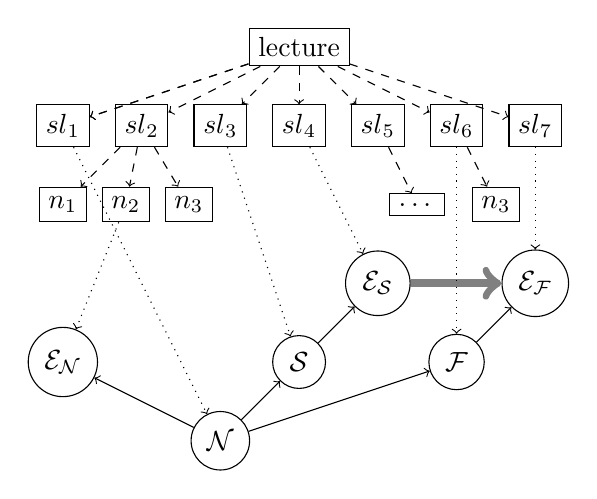
\begin{tikzpicture}
  \begin{scope}[shape=circle]
    \tikzstyle{every node}=[draw]
    \node (N)  at (2,0.5) {$\mathcal{N}$};
    \node (EN) at (0,1.5) {$\mathcal{E_N}$};
    \node (F)  at (5,1.5) {$\mathcal{F}$};
    \node (S)  at (3,1.5) {$\mathcal{S}$};
    \node (EF) at (6,2.5) {$\mathcal{E_F}$};
    \node (ES) at (4,2.5) {$\mathcal{E_S}$};
  \end{scope}
  \draw[->] (N) -- (EN);
  \draw[->] (N) -- (F);
  \draw[->] (N) -- (S);
  \draw[->] (S) -- (ES);
  \draw[->] (F) -- (EF);
  \draw[->,gray,line width=3pt] (ES) -- (EF);
  \begin{scope}
    \tikzstyle{every node}=[draw]
  \node (top) at (3,5.5) {lecture};
  \node (sl1) at (0,4.5) {$\text{sl}_1$};
  \node (sl2) at (1,4.5) {$\text{sl}_2$};
  \node (sl3) at (2,4.5) {$\text{sl}_3$};
  \node (sl4) at (3,4.5) {$\text{sl}_4$};
  \node (an) at (4,4.5) {$\text{sl}_5$};
  \node (sl5) at (5,4.5) {$\text{sl}_6$};
  \node (sl6) at (6,4.5) {$\text{sl}_7$};
  \node (n1) at (0,3.5) {$\text{n}_1$};
  \node (n2) at (.8,3.5) {$\text{n}_2$};
  \node (n3) at (1.6,3.5) {$\text{n}_3$};
  \node (n5) at (4.5,3.5){\ldots};
  \node (n6) at (5.5,3.5) {$\text{n}_3$};
\end{scope}
  \draw[->,dashed] (top) -- (sl1);
  \draw[->,dashed] (top) -- (sl1);
  \draw[->,dashed] (top) -- (sl2);
  \draw[->,dashed] (top) -- (sl3);
  \draw[->,dashed] (top) -- (sl4);
  \draw[->,dashed] (top) -- (an);
  \draw[->,dashed] (top) -- (sl5);
  \draw[->,dashed] (top) -- (sl6);
  \draw[->,dashed] (sl2) -- (n1);
  \draw[->,dashed] (sl2) -- (n2);
  \draw[->,dashed] (sl2) -- (n3);
  \draw[->,dashed] (an) -- (n5);
  \draw[->,dashed] (sl5) -- (n6);

  \draw[->,dotted] (sl1) -- (N);
  \draw[->,dotted] (n2) -- (EN);
  \draw[->,dotted] (sl3) -- (S);
  \draw[->,dotted] (sl4) -- (ES);
  \draw[->,dotted] (sl5) -- (F);
  \draw[->,dotted] (sl6) -- (EF);
\end{tikzpicture}

%%% Local Variables: 
%%% mode: latex
%%% TeX-master: "main"
%%% End: 

% LocalWords:  EF sl
